\documentclass{standalone}
\usepackage{tikz}

\usetikzlibrary{decorations.pathreplacing, angles, quotes}

\begin{document}
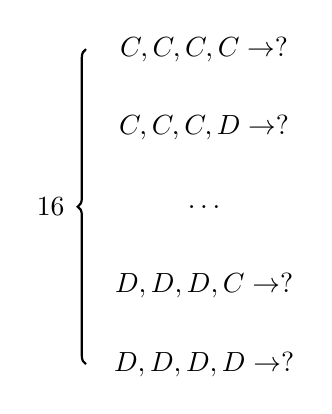
\begin{tikzpicture}
    \node (0) at (0, 0) {$C, C, C, C \rightarrow ?$};
    \node (1) at (0, -1) {$C, C, C, D \rightarrow ?$};
    \node (1) at (0, -2) {$\dots$};
    \node (1) at (0, -3) {$D, D, D, C \rightarrow ?$};
    \node (5) at (0, -4) {$D, D, D, D \rightarrow ?$};

    \draw[thick, decorate,decoration={brace,amplitude=3pt, mirror}]
    (-1.5, 0) -- (-1.5, -4) node[midway, left=4pt] {$16$};
\end{tikzpicture}
\end{document}